\documentclass{article} % JASA requires 12 pt font for manuscripts
%\usepackage{JASA_manu}        % For JASA manuscript formatting

% for citations
\usepackage[authoryear]{natbib} % natbib required for JASA
\usepackage[colorlinks=true, citecolor=blue, linkcolor=blue]{hyperref}

%\definecolor{Blue}{rgb}{0,0,0.5}

\usepackage{amsthm}

% for figures
\usepackage{graphicx}
\usepackage{caption}
\usepackage{subcaption}
\graphicspath{{figures/}}
\newcommand{\hh}[1]{{\color{orange} #1}}
\newcommand{\al}[1]{{\color{red} #1}}

% color in tables
\usepackage{color}

% help with editing and coauthoring
\usepackage{todonotes}

% title formatting
\usepackage[compact,small]{titlesec} 
% page formatting
\usepackage[margin = 1in, landscape]{geometry}
\usepackage[parfill]{parskip}

% line spacing
\usepackage{setspace}
%\doublespace

% For math typsetting
\usepackage{bm}
\usepackage{amstext}
\usepackage{amssymb}
\usepackage{amsmath}
\usepackage{amsfonts}
\usepackage{multirow}
\usepackage{lipsum}

\newtheorem{proposition}{Proposition}
\newtheorem{theorem}{Theorem}
\newtheorem{definition}{Definition}

% A few commands to make typing less tedious
\newcommand{\inv}{\ensuremath{^{-1}}}
\newcommand{\ginv}{\ensuremath{^{-}}}
\newcommand{\trans}{\ensuremath{^\prime}}
\newcommand{\E}{\ensuremath{\mathrm{E}}}
\newcommand{\var}{\ensuremath{\mathrm{Var}}}
\newcommand{\cov}{\ensuremath{\mathrm{Cov}}}
\DeclareMathOperator{\tr}{Trace}
\DeclareMathOperator{\rank}{rank}
\DeclareMathOperator*{\argmin}{arg\,min}


\begin{document}

\section*{Random Intercept}
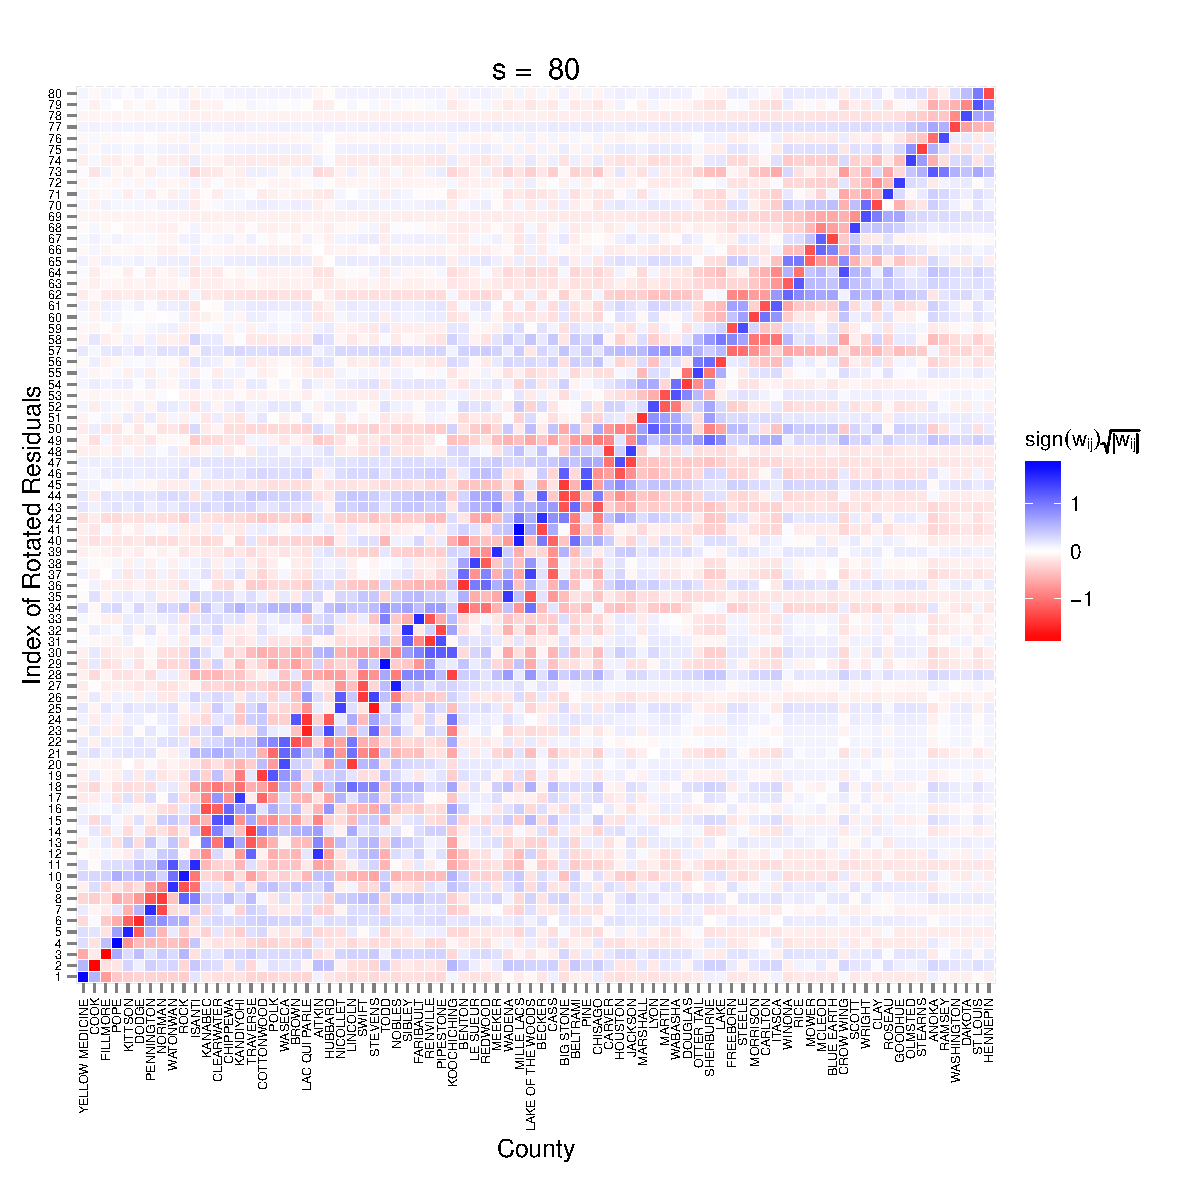
\includegraphics[width=0.5\textwidth]{RandomIntercept_s80.pdf}
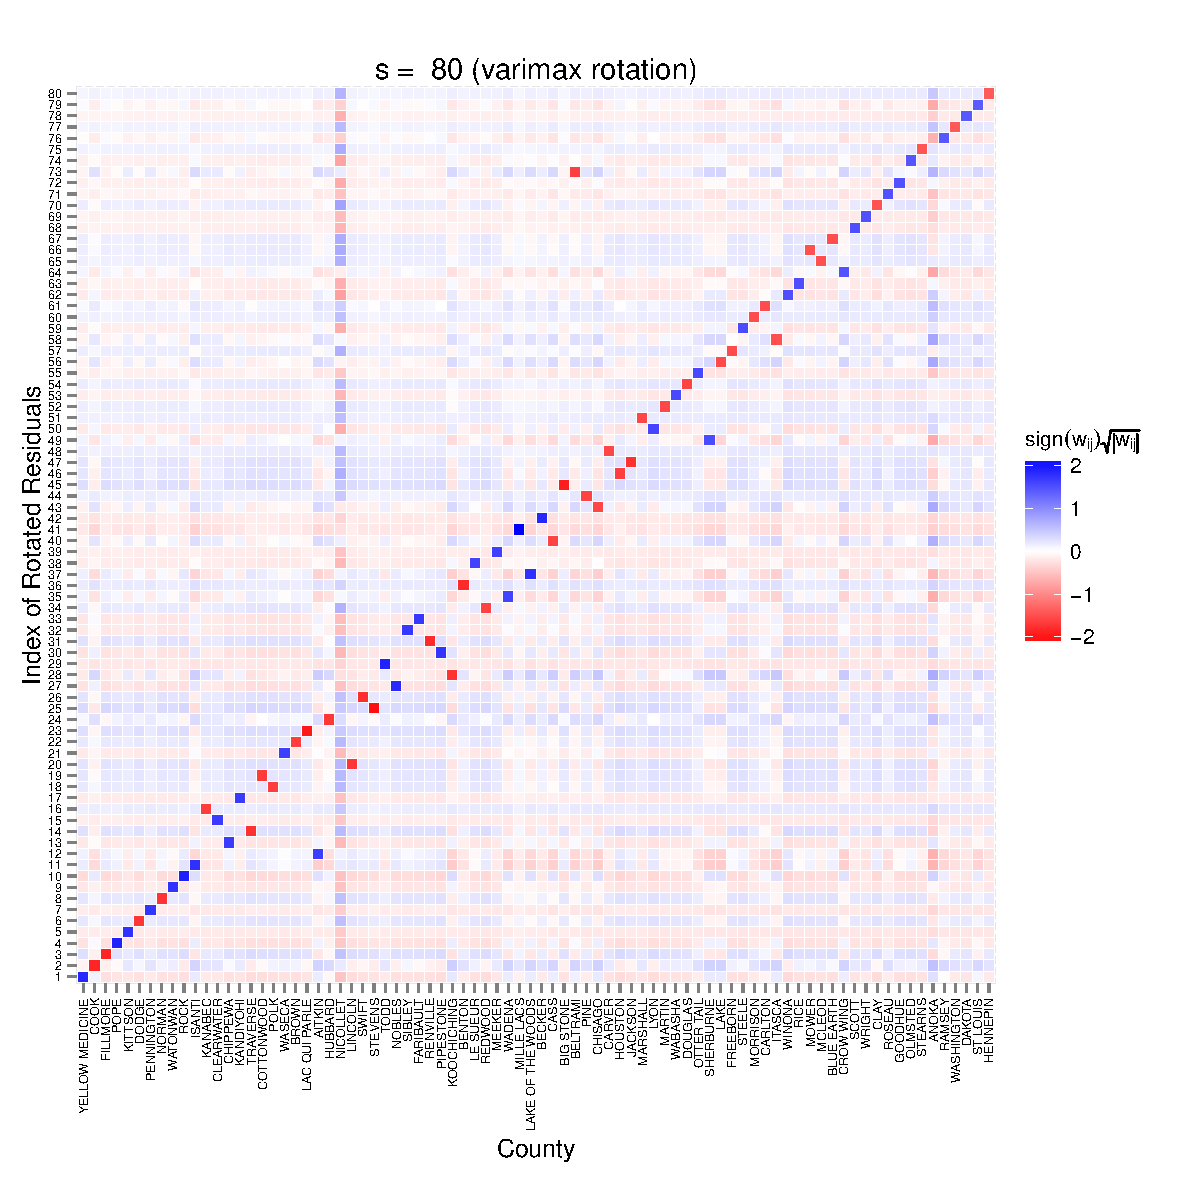
\includegraphics[width=0.5\textwidth]{RandomIntercept_s80_varimax.pdf}

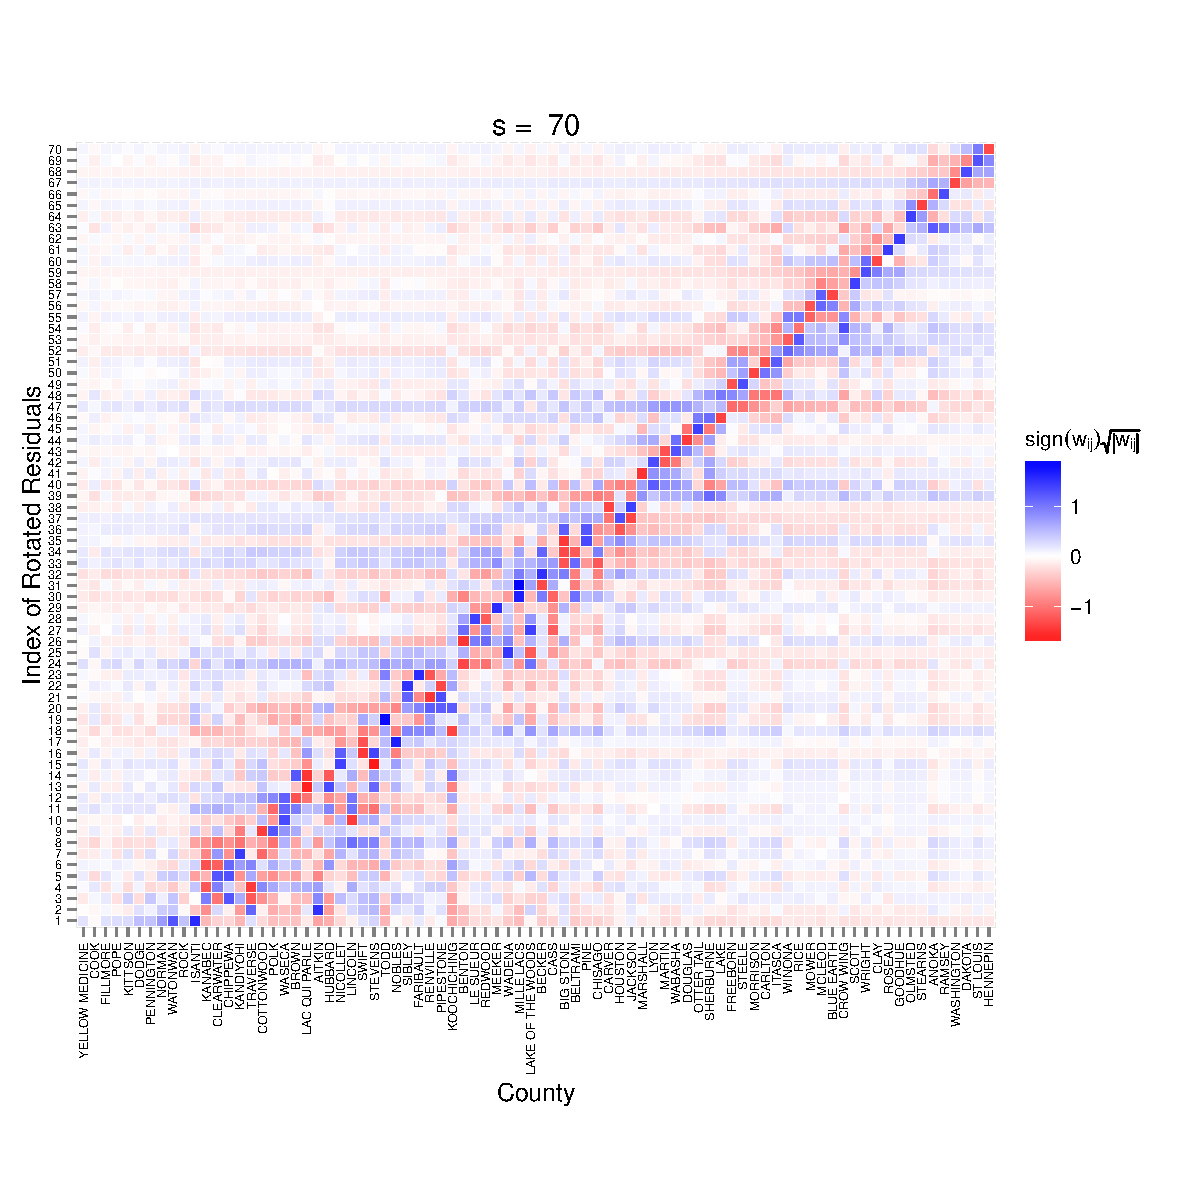
\includegraphics[width=0.5\textwidth]{RandomIntercept_s70.pdf}
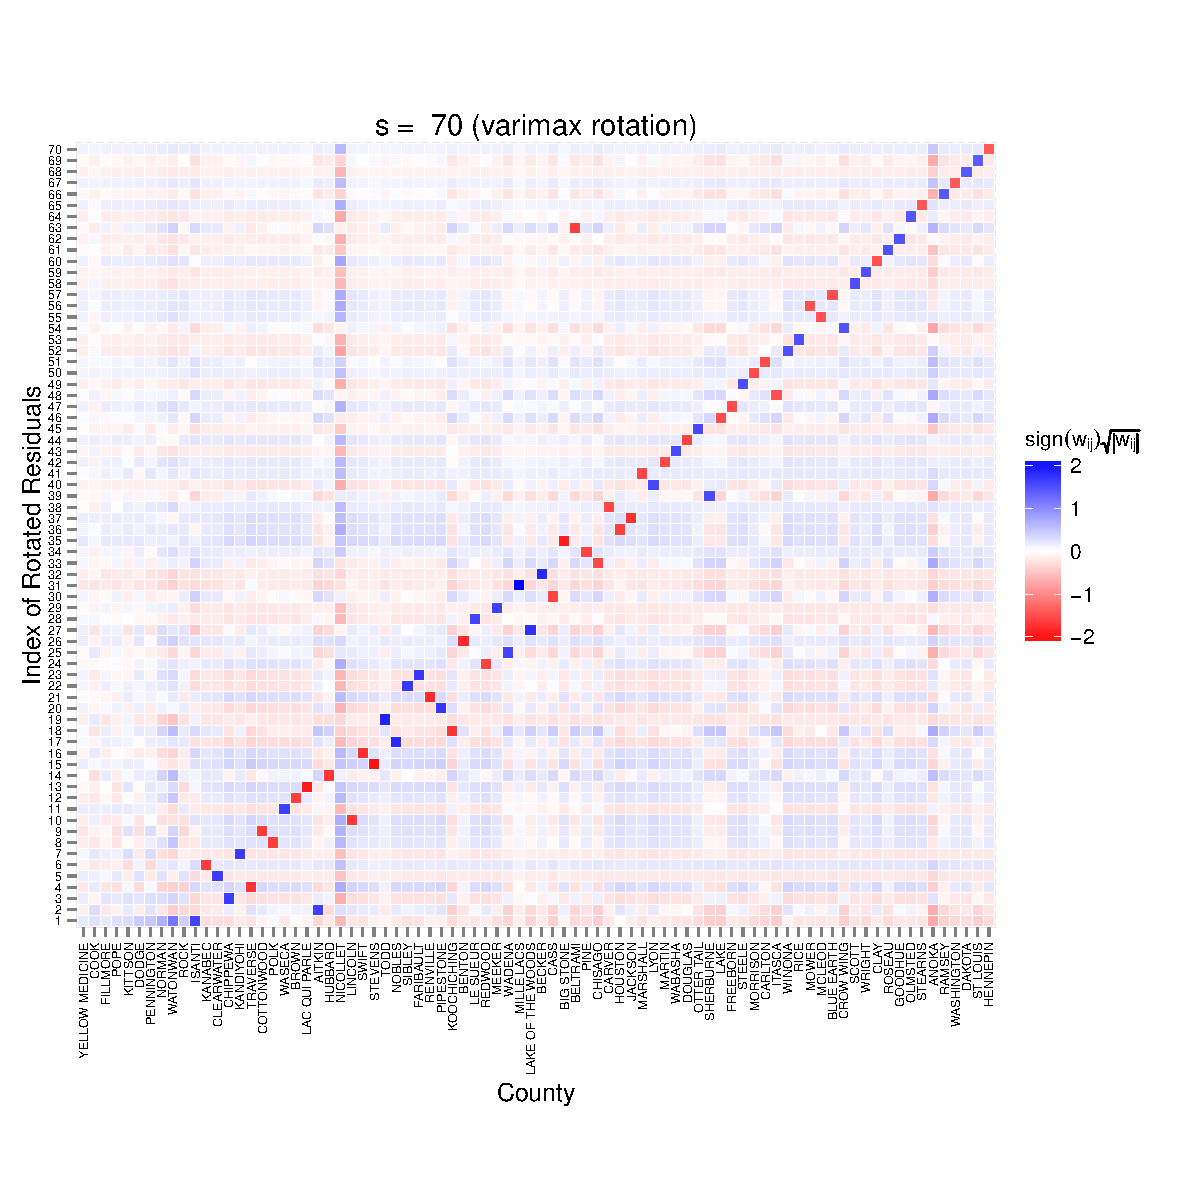
\includegraphics[width=0.5\textwidth]{RandomIntercept_s70_varimax.pdf}

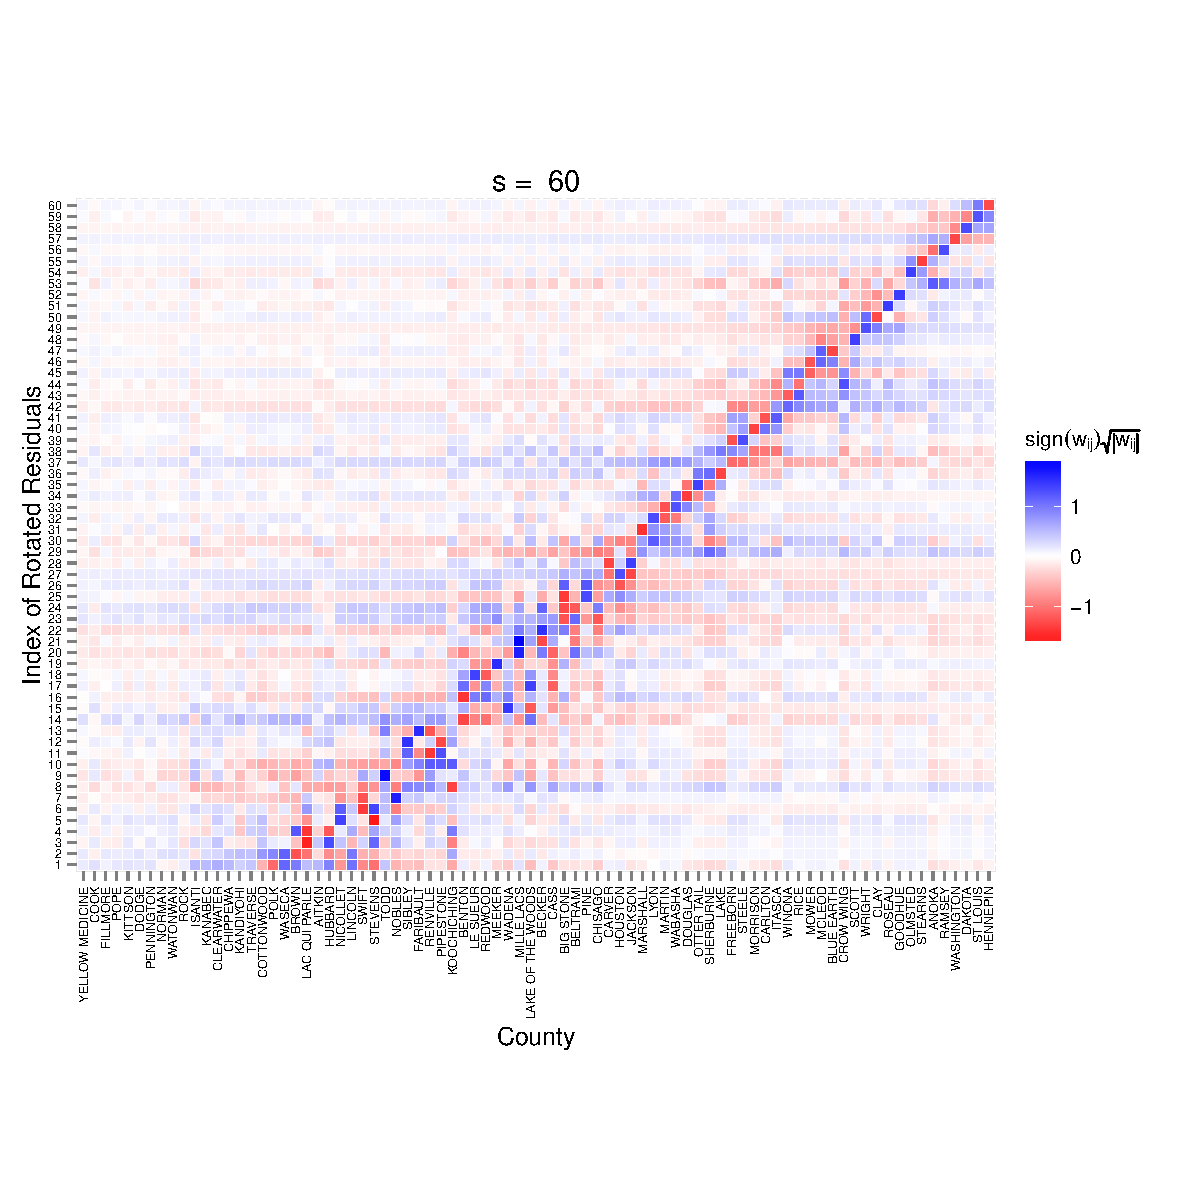
\includegraphics[width=0.5\textwidth]{RandomIntercept_s60.pdf}
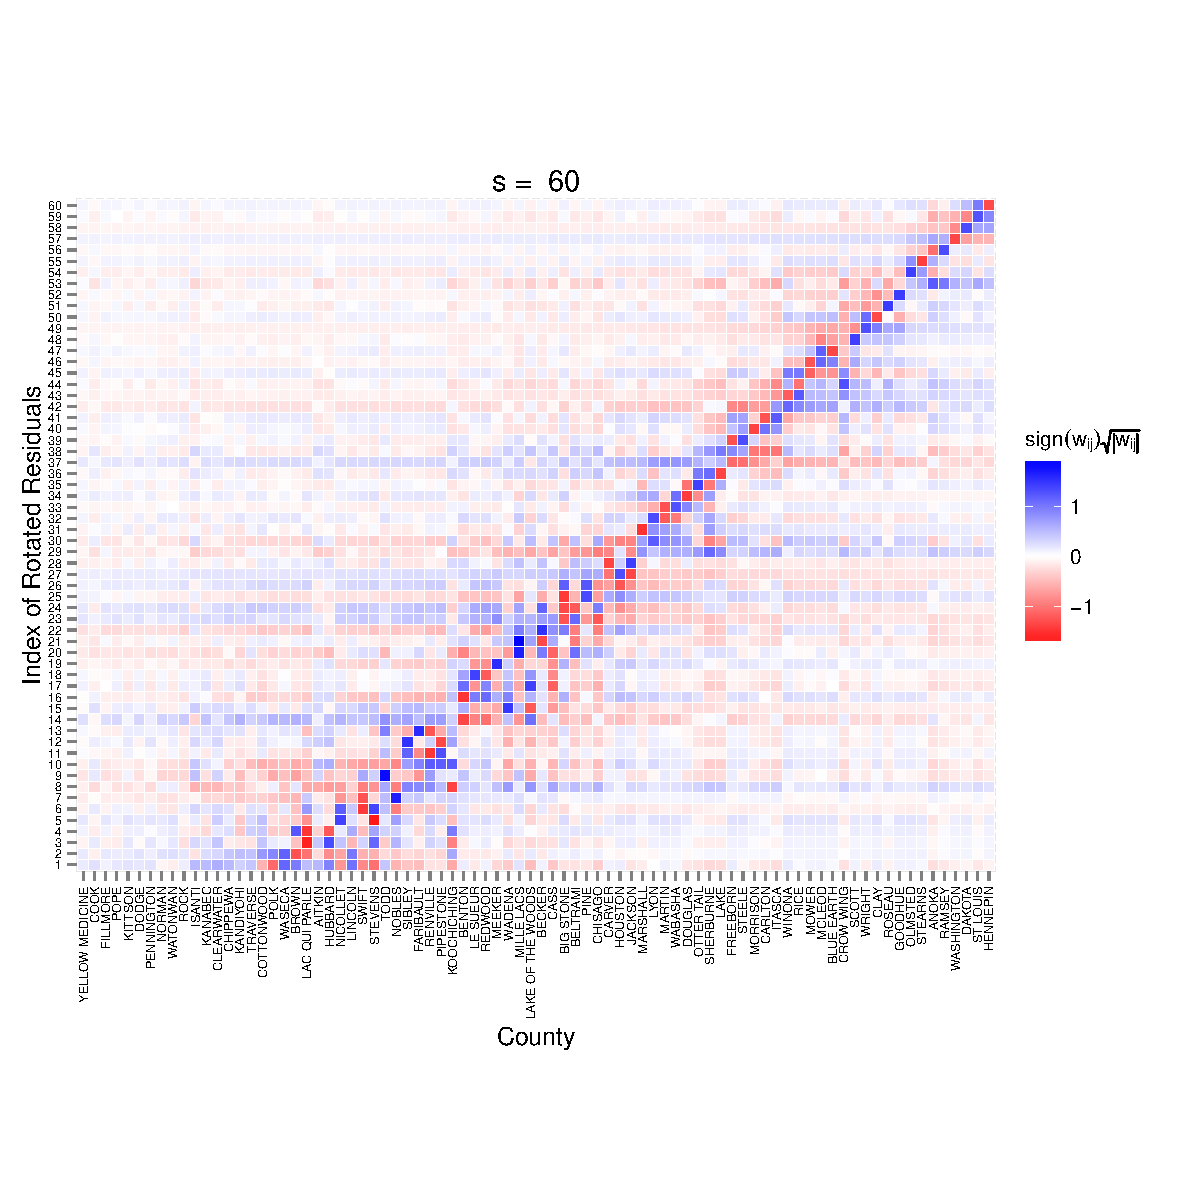
\includegraphics[width=0.5\textwidth]{RandomIntercept_s60_varimax.pdf}

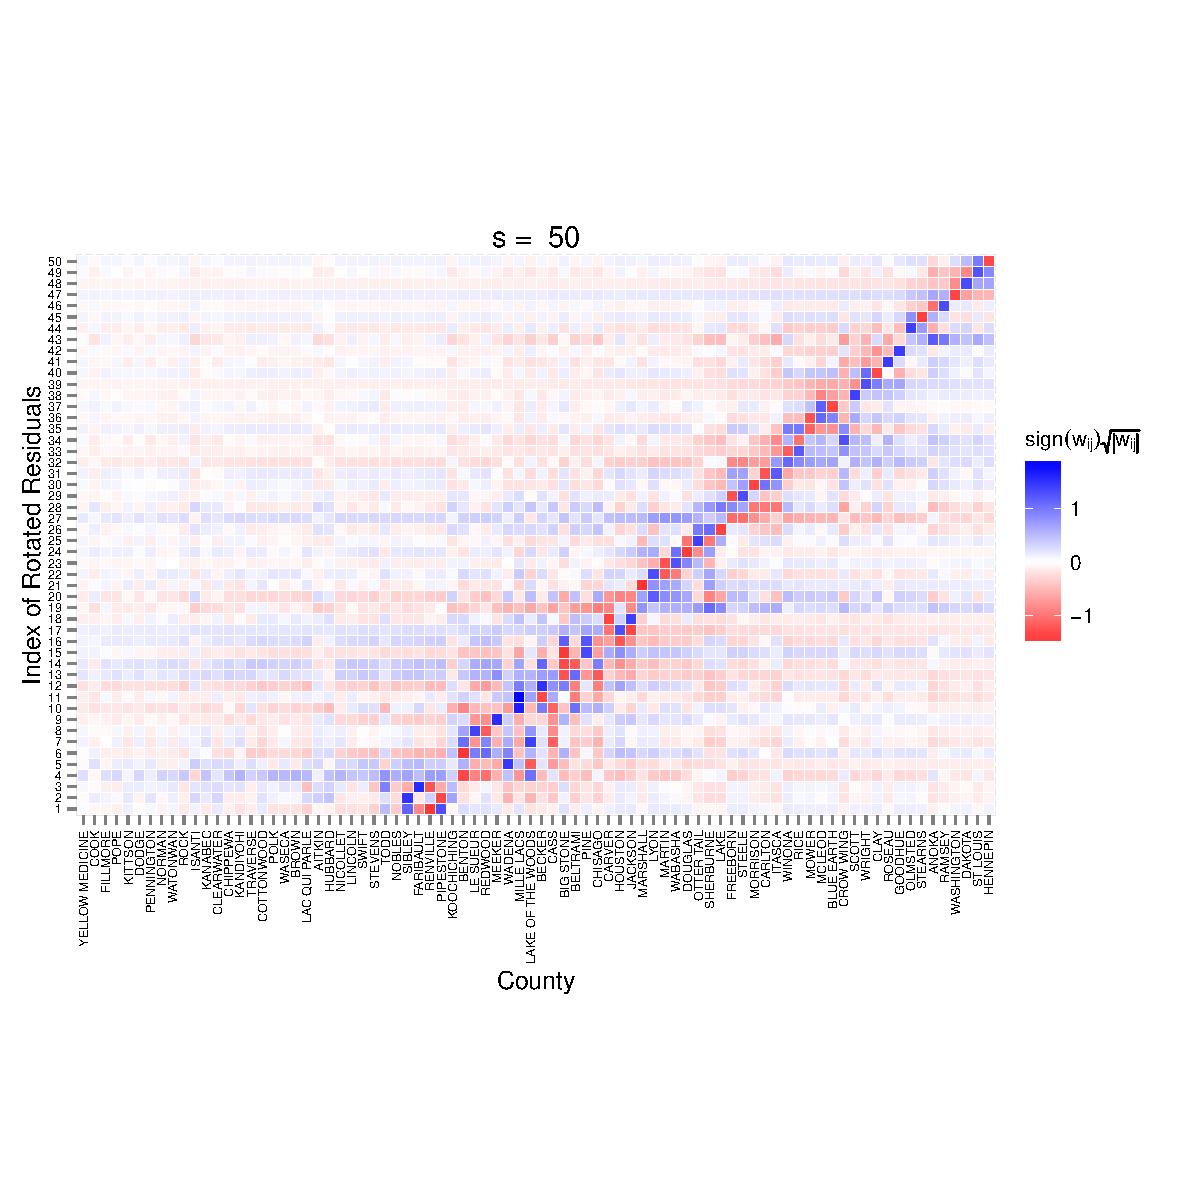
\includegraphics[width=0.5\textwidth]{RandomIntercept_s50.pdf}
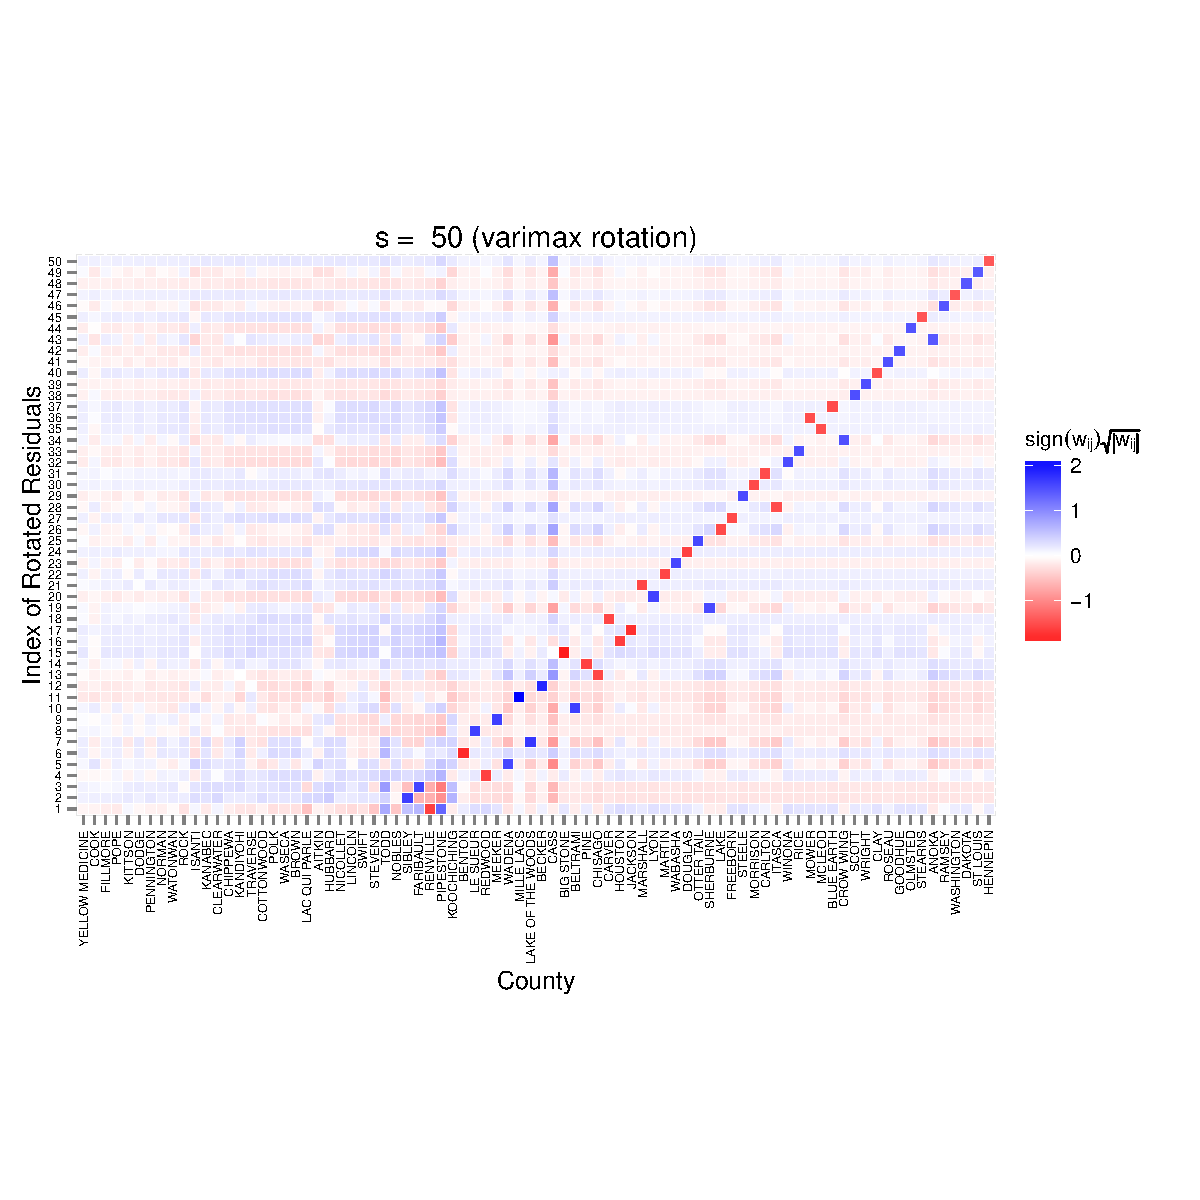
\includegraphics[width=0.5\textwidth]{RandomIntercept_s50_varimax.pdf}


\section*{Random Slope}
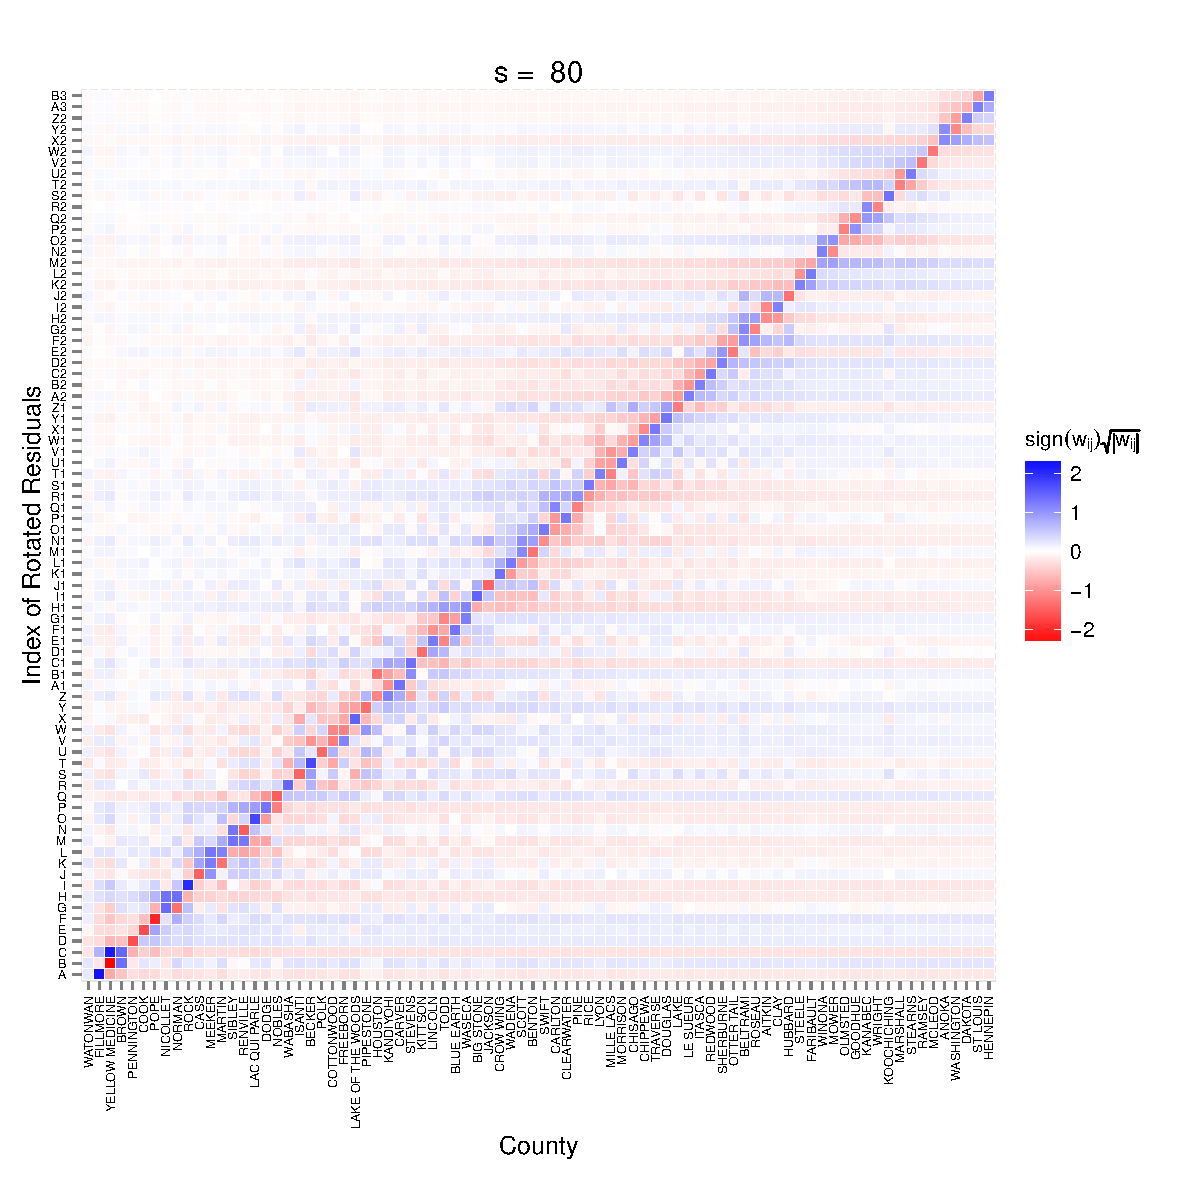
\includegraphics[width=0.5\textwidth]{RandomSlope_s80.pdf}
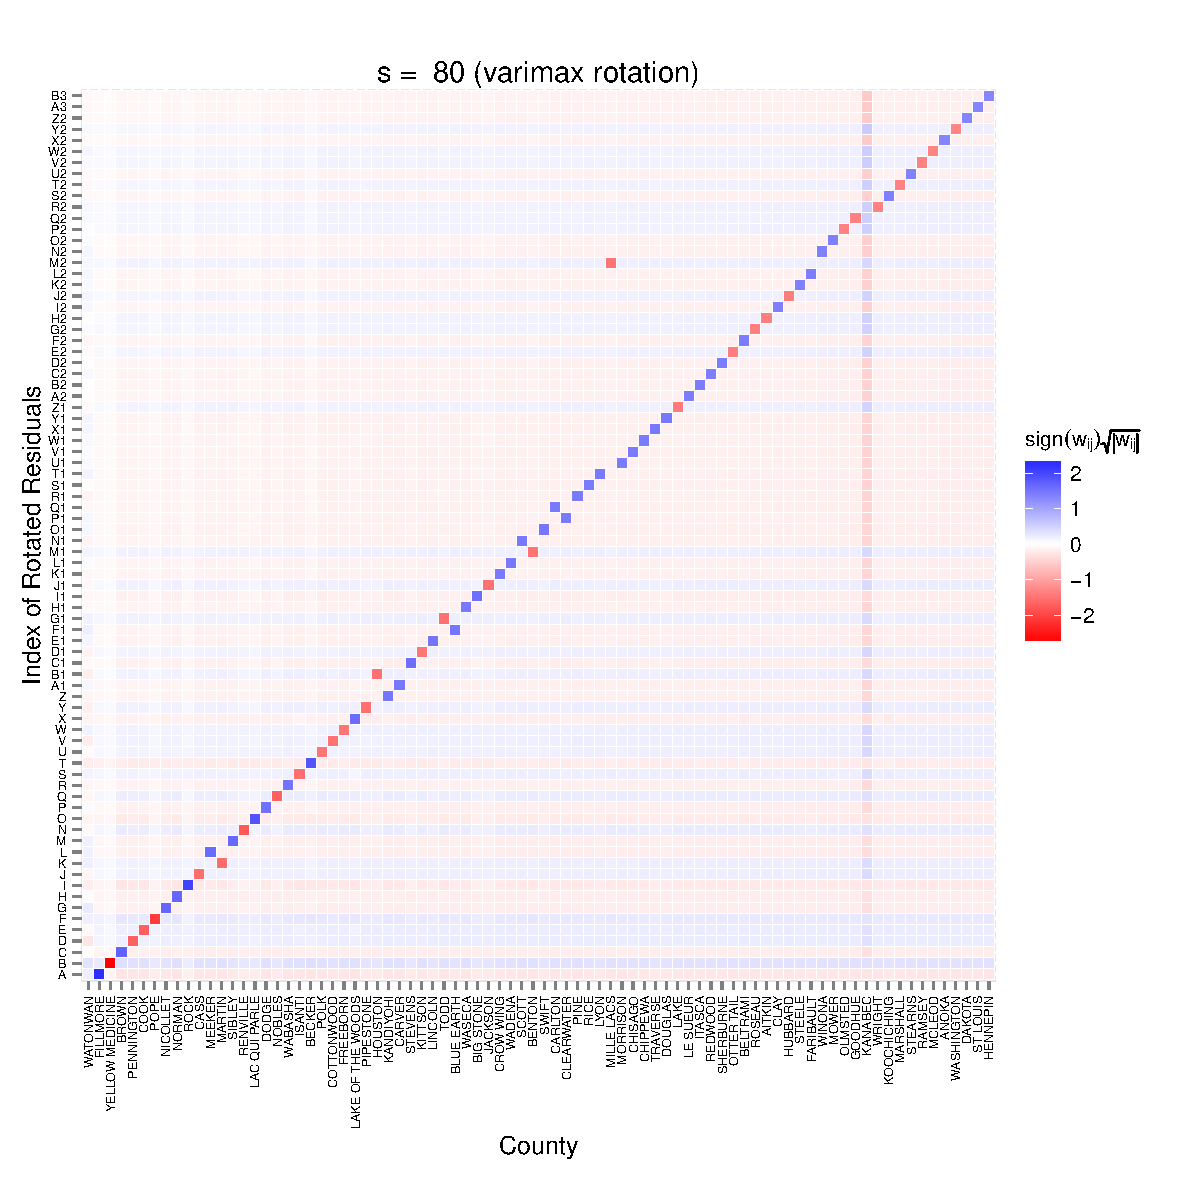
\includegraphics[width=0.5\textwidth]{RandomSlope_s80_varimax.pdf}
 
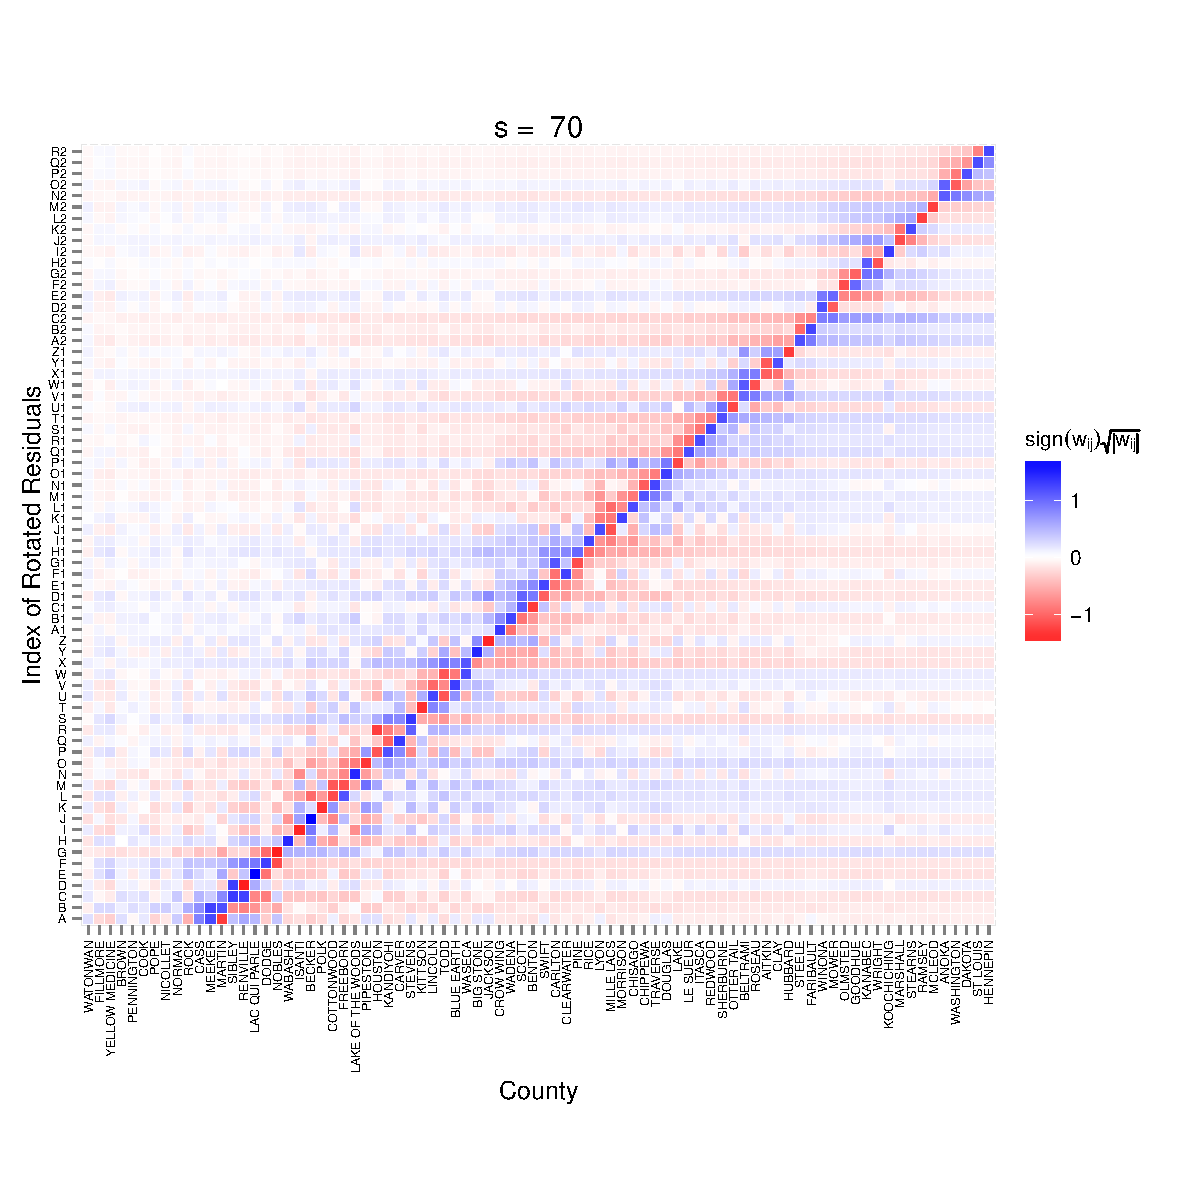
\includegraphics[width=0.5\textwidth]{RandomSlope_s70.pdf}
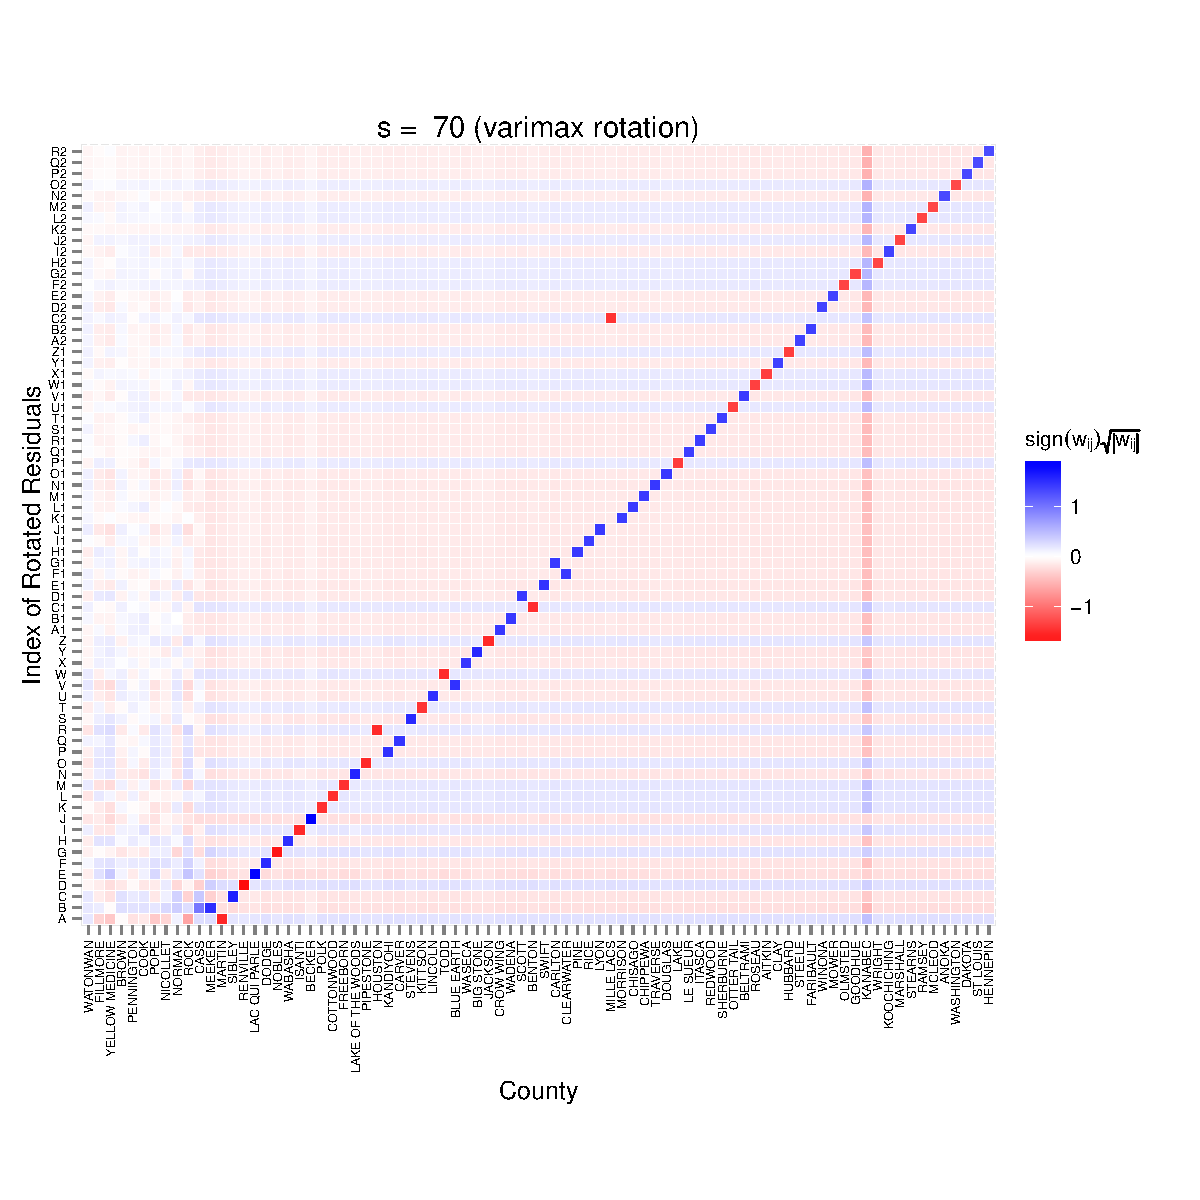
\includegraphics[width=0.5\textwidth]{RandomSlope_s70_varimax.pdf}

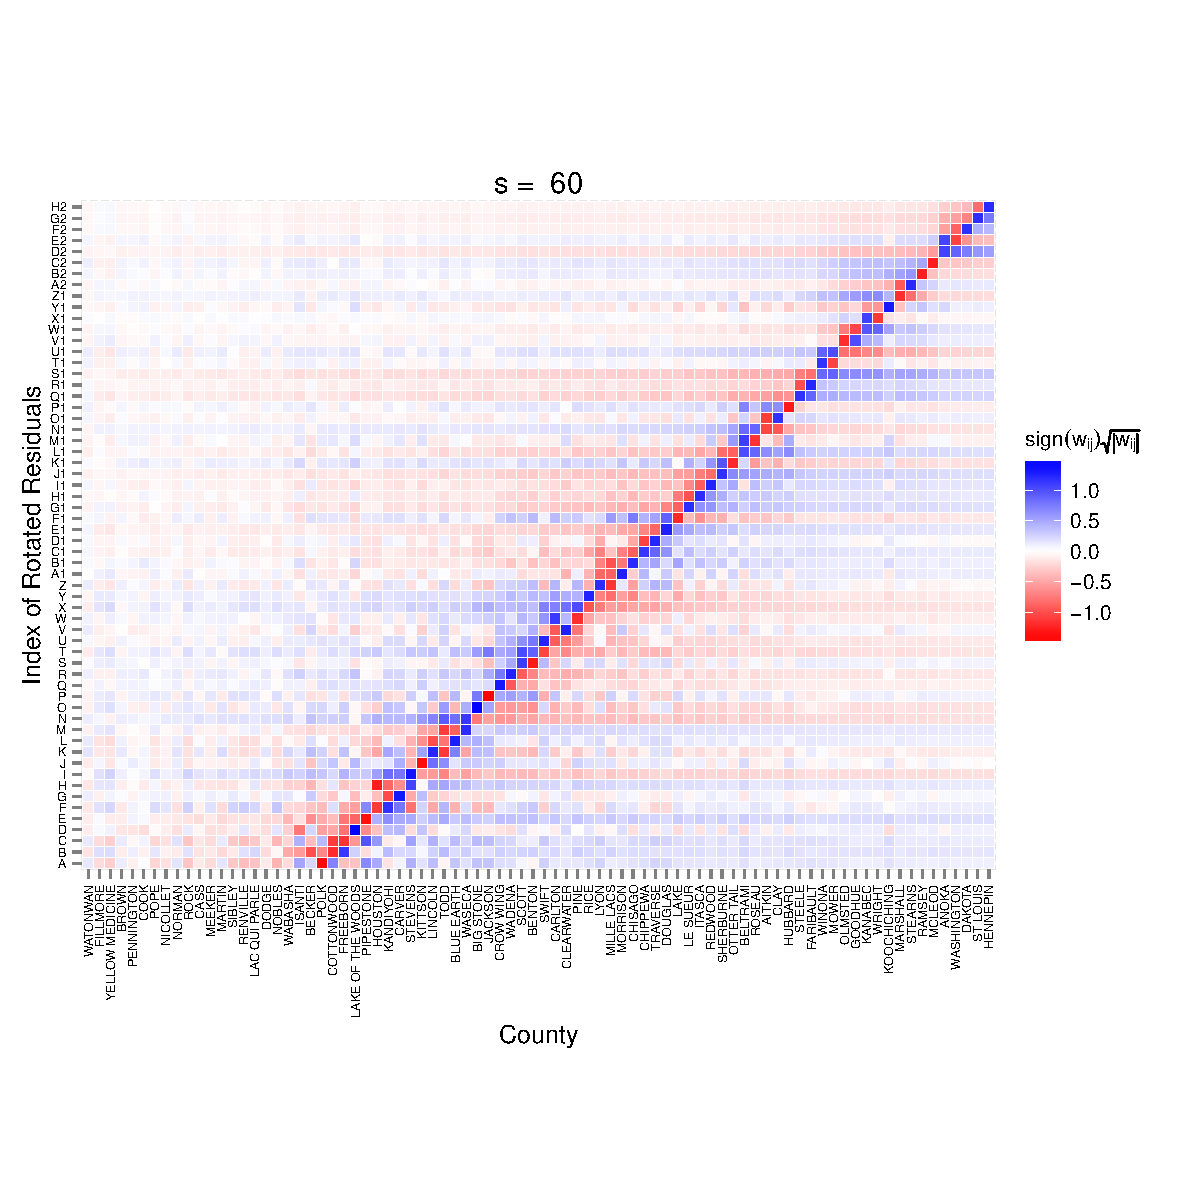
\includegraphics[width=0.5\textwidth]{RandomSlope_s60.pdf}
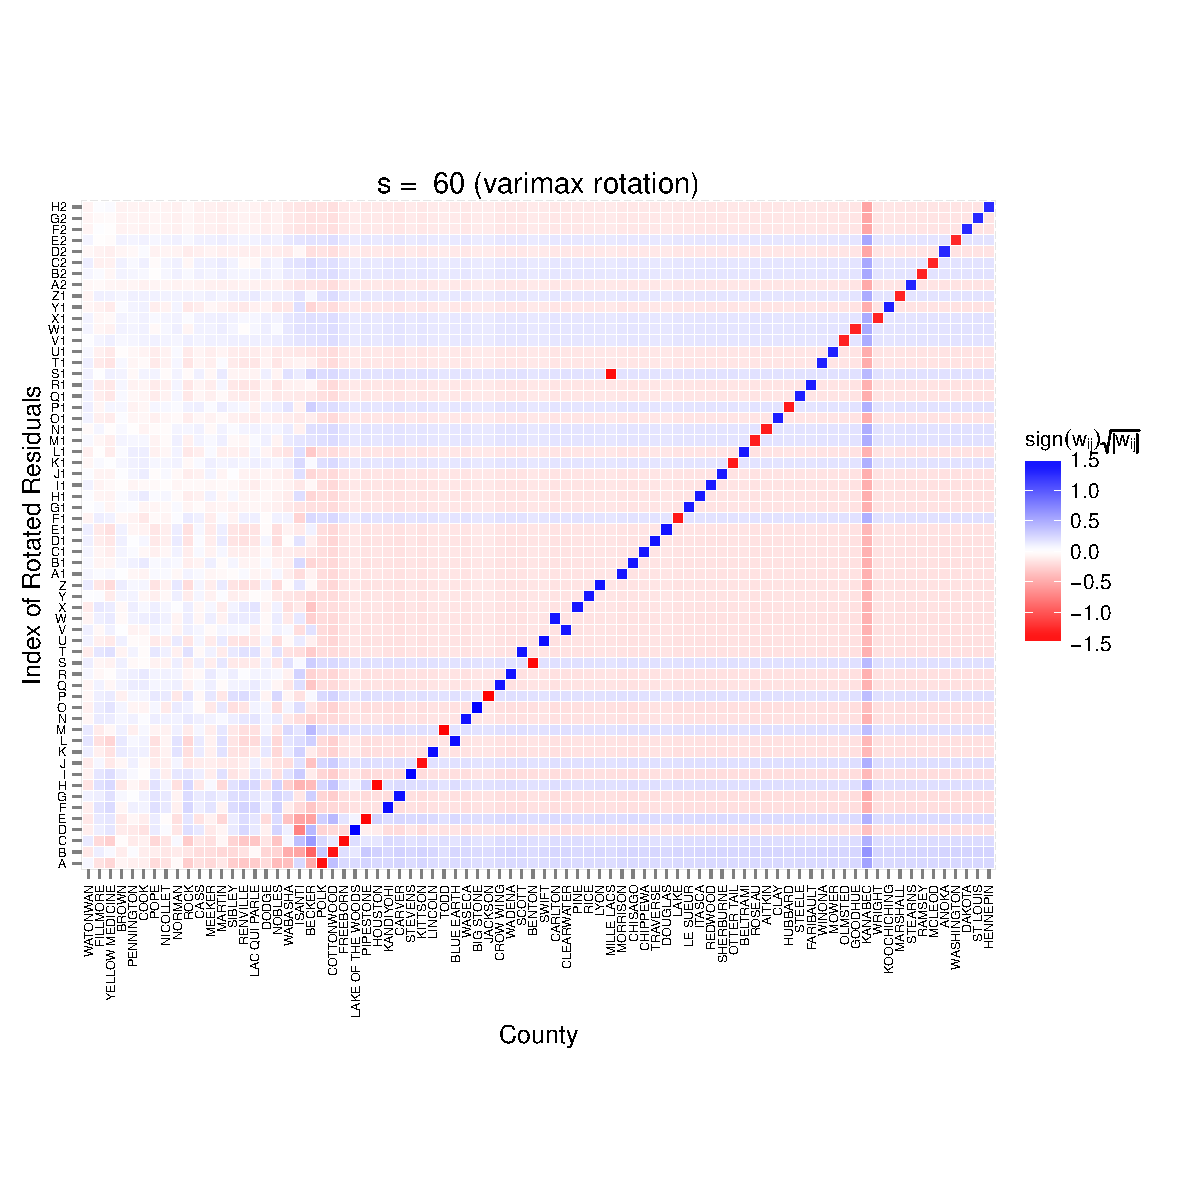
\includegraphics[width=0.5\textwidth]{RandomSlope_s60_varimax.pdf}

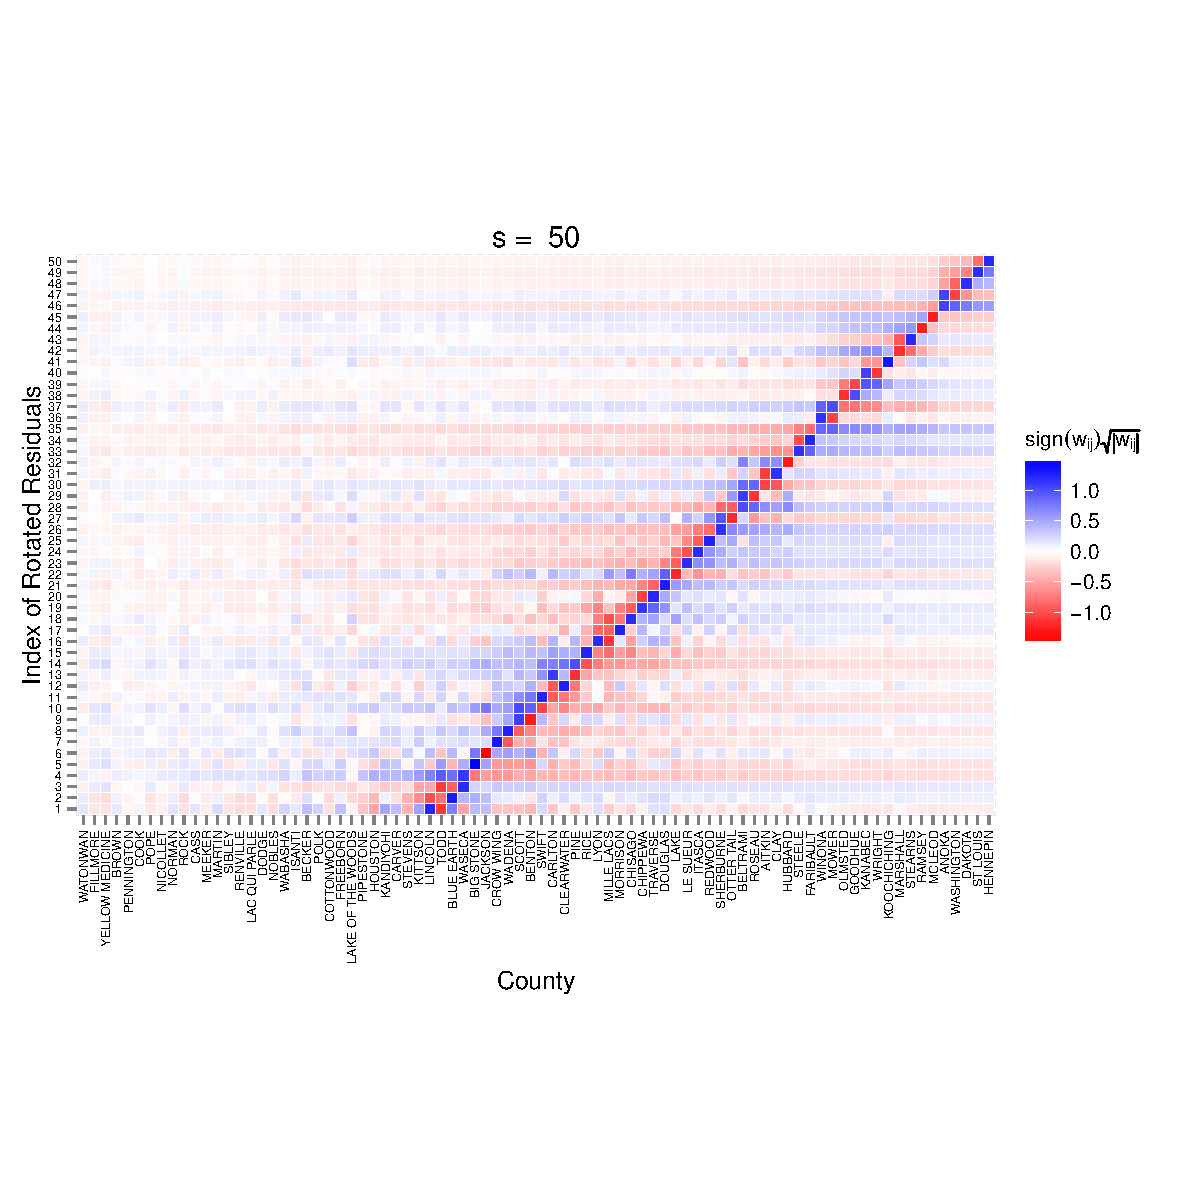
\includegraphics[width=0.5\textwidth]{RandomSlope_s50.pdf}
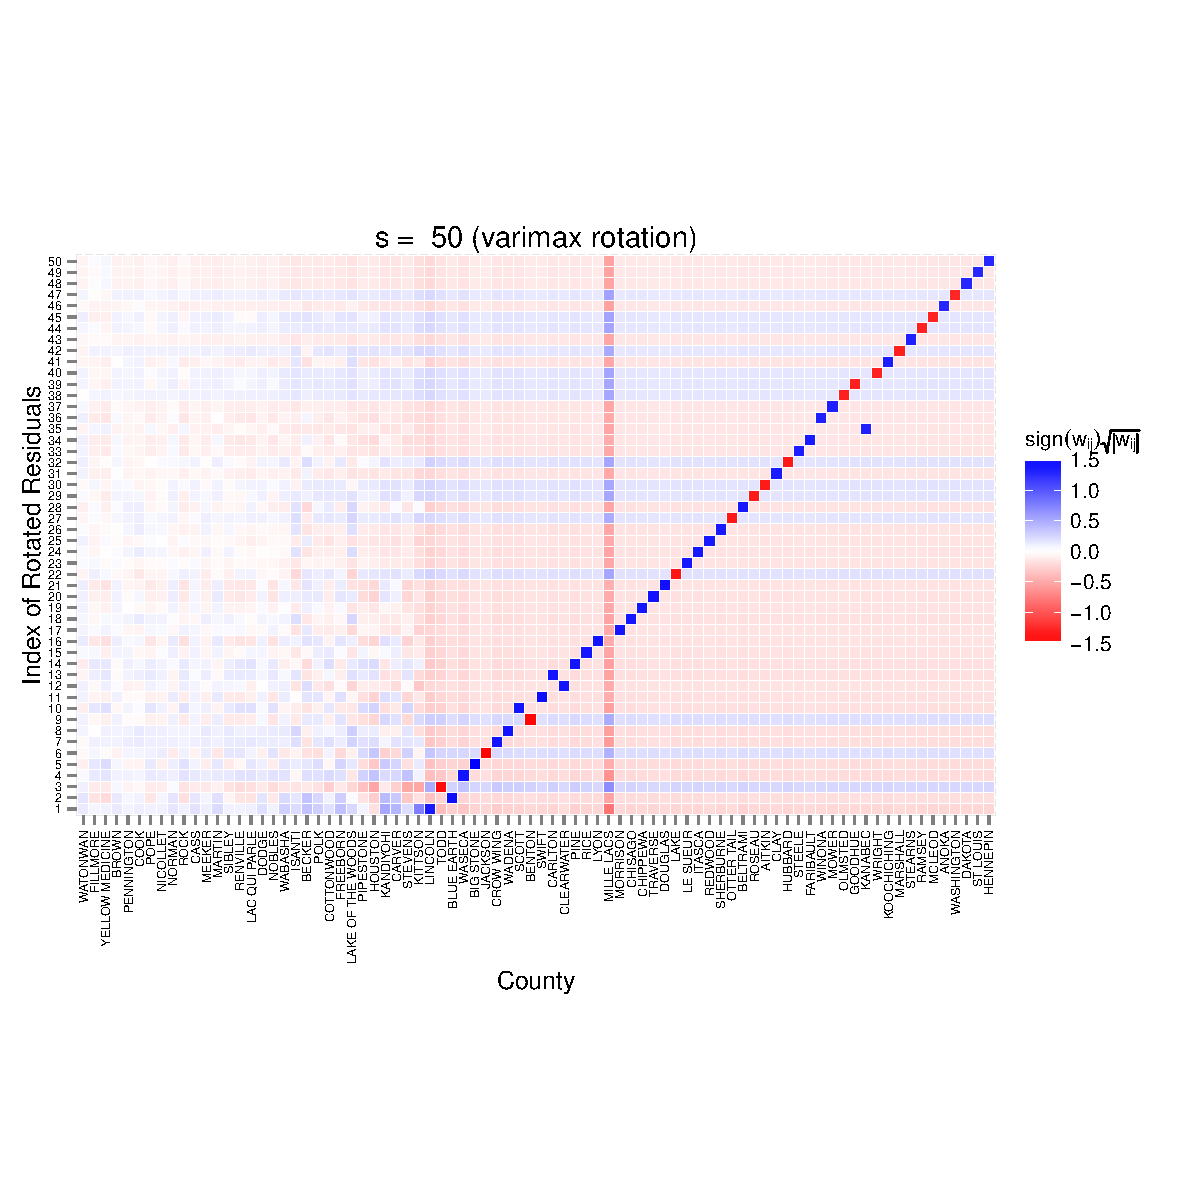
\includegraphics[width=0.5\textwidth]{RandomSlope_s50_varimax.pdf}





\end{document}